% MIT License
% 
% Ankit Maurya
% ankit.dp@bhu.ac.in
% 
% Permission is hereby granted, free of charge, to any person obtaining a copy
% of this software and associated documentation files (the "Software"), to deal
% in the Software without restriction, including without limitation the rights
% to use, copy, modify, merge, publish, distribute, sublicense, and/or sell
% copies of the Software, and to permit persons to whom the Software is
% furnished to do so, subject to the following conditions:
% 
% The above copyright notice and this permission notice shall be included in all
% copies or substantial portions of the Software.
% 
% THE SOFTWARE IS PROVIDED "AS IS", WITHOUT WARRANTY OF ANY KIND, EXPRESS OR
% IMPLIED, INCLUDING BUT NOT LIMITED TO THE WARRANTIES OF MERCHANTABILITY,
% FITNESS FOR A PARTICULAR PURPOSE AND NONINFRINGEMENT. IN NO EVENT SHALL THE
% AUTHORS OR COPYRIGHT HOLDERS BE LIABLE FOR ANY CLAIM, DAMAGES OR OTHER
% LIABILITY, WHETHER IN AN ACTION OF CONTRACT, TORT OR OTHERWISE, ARISING FROM,
% OUT OF OR IN CONNECTION WITH THE SOFTWARE OR THE USE OR OTHER DEALINGS IN THE
% SOFTWARE.







\documentclass[12pt,a4paper]{report}

% Packages
\usepackage{geometry}
\usepackage{fancyhdr}
\usepackage{setspace}
\usepackage{titlesec}
\usepackage{graphicx}
\usepackage{lipsum} 
\usepackage{caption}
\usepackage{listings}
\usepackage{xcolor}
\usepackage{amsmath}
\usepackage{array}
\usepackage{pgfplots}
\lstset{
  language=Python,
  basicstyle=\ttfamily\small,
  keywordstyle=\color{blue},
  commentstyle=\color{green},
  stringstyle=\color{red},
  showstringspaces=false,
  frame=single,
  breaklines=true,
}


% Set page margins
\geometry{top=1in, bottom=1in, left=1in, right=1in}

% Page numbering format
\pagestyle{fancy}
\fancyhf{}
\rfoot{\thepage}
\renewcommand{\headrulewidth}{0pt}

% Chapter and Section formatting
\titleformat{\chapter}[display]
  {\normalfont\fontsize{14}{16}\selectfont\bfseries\centering}{\MakeUppercase{\chaptertitlename}\ \thechapter}{20pt}{\fontsize{14}{16}\selectfont\bfseries}
\titleformat{\section}
  {\normalfont\fontsize{12}{14}\selectfont\bfseries}{\thesection}{1em}{}
\titleformat{\subsection}
  {\normalfont\fontsize{12}{14}\selectfont\bfseries}{\thesubsection}{1em}{}
\titleformat{\subsubsection}
  {\normalfont\fontsize{12}{14}\selectfont\bfseries}{\thesubsubsection}{1em}{}

% Table of Contents formatting
\makeatletter
\renewcommand*\l@chapter[2]{%
  \ifnum \c@tocdepth >\m@ne
    \addpenalty{-\@highpenalty}%
    \vskip 1.0em \@plus\p@
    \setlength\@tempdima{1.5em}%
    \begingroup
      \parindent \z@ \rightskip \@pnumwidth
      \parfillskip -\@pnumwidth
      \leavevmode \bfseries
      \advance\leftskip\@tempdima
      \hskip -\leftskip
      #1\nobreak\hfil \nobreak\hb@xt@\@pnumwidth{\hss #2}\par
      \penalty\@highpenalty
    \endgroup
  \fi}

\renewcommand*\l@section{\@dottedtocline{1}{0em}{2.3em}}
\renewcommand*\l@subsection{\@dottedtocline{2}{2.3em}{3.2em}}
\renewcommand*\l@subsubsection{\@dottedtocline{3}{5.5em}{4.1em}}
\renewcommand*\l@paragraph{\@dottedtocline{4}{8.6em}{5em}}
\renewcommand*\l@subparagraph{\@dottedtocline{5}{12em}{6em}}
\makeatother

% Title Page
\begin{document}
\begin{titlepage}
    \centering
    
    % Title
    {\Huge \bfseries{AI– Algorithms Comparison for Credit Card Fraud Detection Dataset }\par}
    \vspace{0.5cm}
    {\large A report submitted to \par{\textbf{Department of Information Science and Engineering} \par \textbf{JSS Science and Technology University} }\par in partial fulfillment  for the award of the degree of\par}
    {\large\itshape  Bachelor of Engineering\par in\par}
    \vspace{0.5cm}
    {\Large\bfseries \textbf{Computer Science and Business Systems}\par}  % Uncomment this for MCA
    % {\Large\bfseries Master of Science\par}   % Uncomment this for M.sc
    \vspace{0.5cm}
    {\large by\par}
    \vspace{1cm}
    {\Large\bfseries D Amogh (01JST21CB007)\par}
    \vspace{0.2cm}
    {\Large\bfseries Manaswi Kalyan (01JST21CB023)\par}
    \vspace{0.2cm}
     {\Large\bfseries Purvika S Bennur (01JST21CB030)\par}
    \vspace{0.2cm}
     {\Large\bfseries Unnathi S M (01JST21CB048)\par}
    \vspace{1cm}
  { \large Under the supervision of  \par \par Dr. S P Shiva Prakash \par Professor \& HOD \par Department of I S \& E \par JSS S \& T University, Mysuru. }
    \vspace{1cm}
        
    % University Logo
    \includegraphics[width=0.5\textwidth]{jssstulogo.jpg}\\

    \vspace{0.4cm}
    % Department and University
    {\Large\bfseries Department of Information Science and Engineering\par}
    {\Large\bfseries JSS Science and Technology University\par}
   
    {\Large\bfseries 2023-24\par}
\end{titlepage}

% Preliminaries

% Abstract
\chapter*{Abstract}
\addcontentsline{toc}{chapter}{Abstract}
\begin{spacing}{1.5}
 In the highly competitive and data-driven business landscape of today, accurately analyzing financial data is crucial for making well-informed decisions and maintaining a competitive advantage. Machine learning algorithms offer powerful tools that enable organizations to evaluate financial performance, predict future trends, and uncover hidden patterns within data. This report focuses on the application of six prominent machine learning algorithms to evaluate financial data and assess their effectiveness in performance evaluation:

1. Support Vector Machines (SVM)\par
2. K-Nearest Neighbors (KNN)\par
3. Decision Trees (DT)\par
4. Random Forests (RF)\par
5. Artificial Neural Networks (ANN)\par
6. Reinforcement Learning (RL)\par
\end{spacing}
\clearpage






% Table of Contents and List of Figures
\tableofcontents

\clearpage




% Main content
\chapter{Support Vector Machines (SVM)}
% Include your Introduction content here.
A support vector machine (SVM) is a supervised machine learning algorithm that classifies data by finding an optimal line or hyperplane that maximizes the distance between each class in an N-dimensional space.

SVMs are commonly used within classification problems. They distinguish between two classes by finding the optimal hyperplane that maximizes the margin between the closest data points of opposite classes. The number of features in the input data determine if the hyperplane is a line in a 2-D space or a plane in a n-dimensional space. Since multiple hyperplanes can be found to differentiate classes, maximizing the margin between points enables the algorithm to find the best decision boundary between classes. This, in turn, enables it to generalize well to new data and make accurate classification predictions. The lines that are adjacent to the optimal hyperplane are known as support vectors as these vectors run through the data points that determine the maximal margin.

The SVM algorithm is widely used in machine learning as it can handle both linear and nonlinear classification tasks. However, when the data is not linearly separable, kernel functions are used to transform the data higher-dimensional space to enable linear separation. This application of kernel functions can be known as the “kernel trick”, and the choice of kernel function, such as linear kernels, polynomial kernels, radial basis function (RBF) kernels, or sigmoid kernels, depends on data characteristics and the specific use case.The lines that are adjacent to the optimal hyperplane are known as support vectors as these vectors run through the data points that determine the maximal margin.

\begin{figure}
  \centering
\includegraphics[width=0.7\textwidth]{svm.png}
  \caption{SVM Diagram.}
\end{figure}
  

\section{Algorithm}
Support Vector Machine (SVM):

Step 1: Gather the dataset containing labeled data points.

Step 2: Preprocess the data by scaling features if needed.

Step 3: Select a kernel function (e.g., linear, polynomial, or radial basis function).

Step 4: Train the SVM model on the training data by finding the hyperplane that best separates the classes.

Step 5: Evaluate the model on the test data using appropriate metrics (e.g., accuracy, precision, recall).

Step 6: Tune hyperparameters if necessary (e.g., regularization parameter C, kernel parameters).

Step 7: Deploy the trained SVM model for predictions on new data.

\section{Code Snippet}
\begin{lstlisting}
# Split the dataset
X = data.drop('Profitable', axis=1)
y = data['Profitable']
X_train, X_test, y_train, y_test = train_test_split(X, y, test_size=0.2, random_state=42)
 
# Standardize the features
scaler = StandardScaler()
X_train = scaler.fit_transform(X_train)
X_test = scaler.transform(X_test)
 
# Train SVM model
svm_model = SVC(kernel='linear')
svm_model.fit(X_train, y_train)
 
# Predictions and confusion matrix
y_pred = svm_model.predict(X_test)
conf_matrix_svm = confusion_matrix(y_test, y_pred)
print("SVM Confusion Matrix:")
print(conf_matrix_svm)

\end{lstlisting}
\clearpage
\section{Confusion Matrix}
SVM Confusion Matrix\par
\vspace{0.5cm}
Split 0.4
\[
\begin{bmatrix}
  11376 & 5\\
  5 & 7
\end{bmatrix}
\]
Split 0.3
\[
\begin{bmatrix}
  8532 & 6\\
  5 & 2
\end{bmatrix}
\]
Split 0.2
\[
\begin{bmatrix}
  5687 & 4\\
  4 & 2
\end{bmatrix}
\]
Split 0.1
\[
\begin{bmatrix}
  2846 & 0\\
  1 & 2
\end{bmatrix}
\]



\chapter{K-nearest neighbor(KNN)}

While the KNN algorithm can be used for either regression or classification problems, it is typically used as a classification algorithm, working off the assumption that similar points can be found near one another.


For classification problems, a class label is assigned on the basis of a majority vote—i.e. the label that is most frequently represented around a given data point is used. While this is technically considered “plurality voting”, the term, “majority vote” is more commonly used in literature. The distinction between these terminologies is that “majority voting” technically requires a majority of greater than 50\%, which primarily works when there are only two categories. When you have multiple classes—e.g. four categories, you don’t necessarily need 50\% of the vote to make a conclusion about a class; you could assign a class label with a vote of greater than 25\%.However, as a dataset grows, KNN becomes increasingly inefficient, compromising overall model performance. It is commonly used for simple recommendation systems, pattern recognition, data mining, financial market predictions, intrusion detection, and more.

\begin{figure}[ht]
  \centering
 \includegraphics[width=0.7\textwidth]{knn.png}
  \caption{KNN Diagram.}
\end{figure}



\section{Algorithm}
K-nearest neighbor(KNN):\par
Step 1: Load the dataset containing labeled data points.\par
Step 2: Preprocess the data by scaling features if needed.\par
Step 3: Choose the value of K (number of nearest neighbors).\par
Step 4: Calculate the distance between the query instance and all the training samples.\par
Step 5: Sort the distances and select the K nearest neighbors.\par
Step 6: Assign the class label by majority voting among the K neighbors.\par
 Step 7: Evaluate the model's performance using appropriate metrics.\par
 Step 8: Fine-tune the model by adjusting the value of K if necessary.

\section{Code Snippet}
\begin{lstlisting}
from sklearn.neighbors import KNeighborsClassifier
 
# Train KNN model
knn_model = KNeighborsClassifier(n_neighbors=5)
knn_model.fit(X_train, y_train)
# Predictions and confusion matrix
y_pred_knn = knn_model.predict(X_test)
conf_matrix_knn = confusion_matrix(y_test, y_pred_knn)
print("KNN Confusion Matrix:")
print(conf_matrix_knn)

\end{lstlisting}

\section{Confusion Matrix}
KNN Confusion Matrix\par
\vspace{0.5cm}
Split 0.4:
\[
\begin{bmatrix}
  113714 & 10\\
  51 & 148
\end{bmatrix}
\]
Split 0.3:
\[
\begin{bmatrix}
   85289 & 7\\
  39 & 108
\end{bmatrix}
\]
Split 0.2:
\[
\begin{bmatrix}
  56852 & 9\\
  20 & 81
\end{bmatrix}
\]
Split 0.1:
\[
\begin{bmatrix}
  28419 & 7\\
  12 & 43
\end{bmatrix}
\]


\chapter{Random Forest}
Random forest is a commonly-used machine learning algorithm, trademarked by Leo Breiman and Adele Cutler, that combines the output of multiple decision trees to reach a single result. Its ease of use and flexibility have fueled its adoption, as it handles both classification and regression problems.\par
The random forest algorithm is made up of a collection of decision trees, and each tree in the ensemble is comprised of a data sample drawn from a training set with replacement, called the bootstrap sample. Of that training sample, one-third of it is set aside as test data, known as the out-of-bag (oob) sample, which we’ll come back to later. Another instance of randomness is then injected through feature bagging, adding more diversity to the dataset and reducing the correlation among decision trees. Depending on the type of problem, the determination of the prediction will vary. For a regression task, the individual decision trees will be averaged, and for a classification task, a majority vote—i.e. the most frequent categorical variable—will yield the predicted class. Finally, the oob sample is then used for cross-validation, finalizing that prediction. \par
It is a preferred algorithm over others as it reduces time spent on data management and pre-processing tasks. It can be used to evaluate customers with high credit risk, to detect fraud, and option pricing problems. Healthcare: The random forest algorithm has applications within computational biology (link resides outside ibm.com), allowing doctors to tackle problems such as gene expression classification, biomarker discovery, and sequence annotation. 

\begin{figure}
  \centering
\includegraphics[width=0.7\textwidth]{rf.png}
  \caption{Random Forest Diagram.}
\end{figure}




\section{Algorithm}
Random Forest (RF):\par
Step 1: Prepare the dataset containing labeled data points.\par
Step 2: Preprocess the data by handling missing values and encoding categorical variables.\par
Step 3: Create multiple decision trees using bootstrapped samples of the training data.\par
Step 4: At each node of the tree, randomly select a subset of features to split on.\par
Step 5: Grow each tree to its maximum depth without pruning.\par
Step 6: Aggregate the predictions of all trees by taking the mode (for classification) or the mean (for regression).\par
 Step 7: Evaluate the Random Forest model's performance on the test data.\par
Step 8: Fine-tune hyperparameters such as the number of trees and maximum depth if needed.\par 

\section{Code Snippet}
\begin{lstlisting}
from sklearn.ensemble import RandomForestClassifier
# Train Random Forest model
rf_model = RandomForestClassifier(n_estimators=100, random_state=42)
rf_model.fit(X_train, y_train)
# Predictions and confusion matrix
y_pred_rf = rf_model.predict(X_test)
conf_matrix_rf = confusion_matrix(y_test, y_pred_rf)
print("Random Forest Confusion Matrix:")
print(conf_matrix_rf)
\end{lstlisting}

\section{Confusion Matrix}
RF Confusion Matrix\par
\vspace{0.5cm}
Split 0.4:
\[
\begin{bmatrix}
  113713 & 11\\
  46 & 153
\end{bmatrix}
\]
Split 0.3:
\[
\begin{bmatrix}
  85291 & 5\\
  35 & 112
\end{bmatrix}
\]
Split 0.2:
\[
\begin{bmatrix}
  56855 & 6\\
  21 & 80
\end{bmatrix}
\]
Split 0.1:
\[
\begin{bmatrix}
  28421 & 5\\
  11 & 44
\end{bmatrix}
\]


\chapter{Decision Tree}
A decision tree is a non-parametric supervised learning algorithm, which is utilized for both classification and regression tasks. It has a hierarchical, tree structure, which consists of a root node, branches, internal nodes and leaf nodes.\par 
Decision Tree is a versatile supervised learning algorithm primarily used for classification and regression tasks.A Decision Tree is a supervised machine learning algorithm used for both classification and regression tasks. It operates by recursively splitting the data into subsets based on the most significant feature at each node, chosen to maximize the separation of classes or minimize prediction error. This process creates a tree-like model of decisions, where each internal node represents a feature, each branch represents a decision rule, and each leaf node represents an outcome. Decision Trees are easy to understand and interpret, handle both numerical and categorical data, and require minimal data preprocessing. However, they can be prone to overfitting, especially with complex trees, which can be mitigated by techniques such as pruning or setting a maximum depth.

\begin{figure}[ht]
  \centering
 \includegraphics[width=0.7\textwidth]{dt.png}
  \caption{Decision tree Diagram.}
\end{figure}


\section{Algorithm}
Decision Tree (DT): \par
Step 1: Load the dataset containing labeled data points.\par
 Step 2: Preprocess the data by handling missing values and encoding categorical variables.\par
  Step 3: Choose a splitting criterion (e.g., Gini impurity, information gain).\par
  Step 4: Recursively partition the feature space into smaller subsets using the selected splitting criterion.\par
  Step 5: Stop splitting when a stopping criterion is met (e.g., maximum depth, minimum samples per leaf).\par
  Step 6: Assign a class label to each leaf node based on the majority class of training instances in that node.\par
  Step 7: Evaluate the Decision Tree model's performance on the test data.\par
  Step 8: Prune the tree if necessary to avoid overfitting.\par
  

\section{Code Snippet}
\begin{lstlisting}
from sklearn.tree import DecisionTreeClassifier
# Train Decision Tree model
dt_model = DecisionTreeClassifier(random_state=42)
dt_model.fit(X_train, y_train)
# Predictions and confusion matrix
y_pred_dt = dt_model.predict(X_test)
conf_matrix_dt = confusion_matrix(y_test, y_pred_dt)
print("Decision Tree Confusion Matrix:")
print(conf_matrix_dt)
\end{lstlisting}

\section{Confusion Matrix}
DT Confusion Matrix\par
\vspace{0.5cm}
Split 0.4
\[
\begin{bmatrix}
  113675 & 49\\
 54 & 145
\end{bmatrix}
\]
Split 0.3
\[
\begin{bmatrix}
 85267 & 29\\
  38 & 109
\end{bmatrix}
\]
Split 0.2
\[
\begin{bmatrix}
  56836 & 25\\
  23 & 78
\end{bmatrix}
\]
Split 0.1
\[
\begin{bmatrix}
  28414 & 12\\
  13 & 42
\end{bmatrix}
\]

\chapter{Artificial Neural Network (ANN)}
Artificial Neural Network (ANN) is a computational model inspired by the structure and functioning of the human brain's neural networks Artificial Neural Networks are capable of learning complex patterns and relationships in data, making them suitable for a wide range of tasks, including classification, regression, image recognition, natural language processing, and more. \par
A neural network is a machine learning program, or model, that makes decisions in a manner similar to the human brain, by using processes that mimic the way biological neurons work together to identify phenomena, weigh options and arrive at conclusions. \par
Every neural network consists of layers of nodes, or artificial neurons—an input layer, one or more hidden layers, and an output layer. Each node connects to others, and has its own associated weight and threshold. If the output of any individual node is above the specified threshold value, that node is activated, sending data to the next layer of the network. Otherwise, no data is passed along to the next layer of the network. \par
Input Layer:
As the name suggests, it accepts inputs in several different formats provided by the programmer.\par
Hidden Layer:
The hidden layer presents in-between input and output layers. It performs all the calculations to find hidden features and patterns.\par
Output Layer:
The input goes through a series of transformations using the hidden layer, which finally results in output that is conveyed using this layer.\par

\begin{figure}
  \centering
\includegraphics[width=0.7\textwidth]{ann.png}
  \caption{Artificial Neural Networks Diagram.}
\end{figure}

\section{Algorithm}
Artificial Neural Networks (ANN): \par
Step 1: Load the dataset containing input-output pairs.\par
 Step 2: Preprocess the data by scaling features, encoding categorical variables, and splitting into training and test sets.\par
  Step 3: Design the architecture of the neural network (number of layers, number of neurons per layer, activation functions).\par
  Step 4: Compile the model by specifying the loss function, optimizer, and evaluation metrics.\par
   Step 5: Train the model on the training data using backpropagation and gradient descent.\par
   Step 6: Evaluate the model's performance on the test data.\par
  Step 7: Fine-tune hyperparameters such as learning rate and batch size if needed.\par
  Step 8: Deploy the trained neural network for making predictions on new data.\par

\section{Code Snippet}
\begin{lstlisting}
    # Feature selection
    X = df.drop(columns=['Class'])
    y = df['Class']

    # Training-testing ratios
    ratios = [0.4, 0.3, 0.2, 0.1]
    # Initialize the ANN
    model = Sequential()
    model.add(Dense(units=64, activation='relu', input_dim=X_train.shape[1]))
    model.add(Dense(units=32, activation='relu'))
    model.add(Dense(units=1, activation='sigmoid'))

    # Compile the ANN
    model.compile(optimizer='adam', loss='binary_crossentropy', metrics=['accuracy'])

    # Train the ANN
    model.fit(X_train, y_train, epochs=50, batch_size=32, verbose=1)

    # Predictions
    y_pred = model.predict(X_test)
    y_pred = (y_pred > 0.5).astype(int)

    # Confusion matrix
    cm = confusion_matrix(y_test, y_pred)
    print(f"Confusion Matrix for split {ratio}:\n", cm)
    results[ratio] = {'precision': precision_q, 'accuracy': accuracy_q, 'recall': recall_q, 'f1': f1_q}
\end{lstlisting}
\clearpage
\section{Confusion Matrix}
ANN Confusion Matrix for: \par
 \vspace{0.5cm}

Split 0.4:
\[
\begin{bmatrix}
  113697 & 27\\
  45 & 154
\end{bmatrix}
\]
 \vspace{0.5cm}
Split 0.3:
\[
\begin{bmatrix}
  85278 & 18\\
  32 & 115
\end{bmatrix}
\]
Split 0.2:
 \vspace{0.5cm}
\[
\begin{bmatrix}
  56845 & 16\\
  23 & 78
\end{bmatrix}
\]
Split 0.1:
 \vspace{0.5cm}
\[
\begin{bmatrix}
  28419 & 7\\
  13 & 42
\end{bmatrix}
\]


\chapter{Reinforcement Learning}
Reinforcement Learning (RL), specifically Q-learning, is a type of machine learning algorithm used for sequential decision-making tasks.Reinforcement Learning (RL) is a type of machine learning paradigm where an agent learns to make sequential decisions through interaction with an environment to maximize cumulative rewards. At each time step, the agent takes an action based on its current state and receives feedback in the form of a reward and the next state. The goal of the agent is to learn a policy, which is a mapping from states to actions, that maximizes the expected cumulative reward over time. RL differs from supervised learning in that it learns from feedback in the form of rewards rather than explicit labels.\par 
Key components of RL include the agent, environment, state space, action space, reward function, and learning algorithm. RL techniques such as Q-Learning, Policy Gradient methods, and Deep Q Networks (DQN) have been successfully applied to various tasks including game playing, robotics, and autonomous systems. However, RL comes with challenges such as exploration-exploitation trade-off, credit assignment problem, and sample inefficiency, which researchers continue to address through advancements in algorithms and techniques.

\begin{figure}[ht]
  \centering
 \includegraphics[width=0.7\textwidth]{rl.jpg}
  \caption{Reinforcement Learning Diagram.}
\end{figure}


\section{Algorithm}
Step 1: Initialize Q-table with zeros or random values.\par
Step 2: Choose an action based on the current state using an exploration-exploitation strategy (e.g., epsilon-greedy).\par
Step 3: Perform the chosen action and observe the reward and next state.\par
 Step 4: Update the Q-value of the current state-action pair using the Q-learning equation.\par
  Step 5: Repeat steps 2-4 for a fixed number of episodes or until convergence.\par
   Step 6: Optionally, apply techniques like experience replay and target networks for stability.\par
   Step 7: Evaluate the learned policy on a separate test environment to assess its performance.\par
 Step 8: Fine-tune hyperparameters such as learning rate, discount factor, and exploration rate if needed.\par

\section{Code Snippet}
\begin{lstlisting}
# Pseudo-code example for Q-Learning in financial context
# Define environment and state-action space
states = [...]  # define your states
actions = [...]  # define your actions
q_table = np.zeros((len(states), len(actions)))
# Parameters
learning_rate = 0.1
discount_factor = 0.95
epsilon = 0.1
# Training loop
for episode in range(1000):
    state = initial_state  # initialize starting state
    done = False    
    while not done:
        if np.random.uniform(0, 1) < epsilon:
            action = random.choice(actions)  # Explore
        else:
            action = np.argmax(q_table[state])  # Exploit
        new_state, reward, done = take_action(state, action)
        # Update Q-Table
        q_table[state, action] = q_table[state, action] + learning_rate * (reward + discount_factor * np.max(q_table[new_state]) - q_table[state, action])
        state = new_state
# Using the trained Q-Table for making predictions
def make_prediction(state):
    return np.argmax(q_table[state])
\end{lstlisting}
\clearpage

\section{Confusion Matrix}
QL Confusion Matrix\par
Split 0.4
\[
\begin{bmatrix}
  111614 & 2118\\
  188 & 3
\end{bmatrix}
\]
Split 0.3
\[
\begin{bmatrix}
  84445 & 862\\
  136 & 0
\end{bmatrix}
\]
Split 0.2
\[
\begin{bmatrix}
  56341 & 523\\
  97 & 1
\end{bmatrix}
\]
Split 0.1
\[
\begin{bmatrix}
  28365 & 70\\
  46 & 0
\end{bmatrix}
\]


% Results and Discussion
\chapter{Results }
% Include your Results and Discussion content here.
\section{Precision Table}
\begin{table}[!ht]
\centering
\begin{tabular}{|c|c|c|c|c|c|c|}
  \hline
  Split & SVM & KNN & RF & DT & ANN & RL \\
  \hline
  0.4 & 0.5833  & 0.9367 & 0.9329 & 0.7474 & 0.8508 & 0.7179 \\
  \hline
  0.3 & 0.2500 & 0.9391 & 0.9573 & 0.7899 & 0.8647 & 0.7453 \\
  \hline
  0.2 & 0.3333 & 0.9000 & 0.9302 & 0.7573 & 0.8298 & 0.7621 \\
  \hline
  0.1 & 1.0000 & 0.8600 & 0.8980 & 0.7778 & 0.8571 & 0.5461 \\
  \hline
  Average & 0.5417 & 0.909 & 0.9296 & 0.7681 & 0.8506 & 0.6928 \\
  \hline
\end{tabular}
\caption{Precision Table for various training testing ratio}
\label{tab:results}
\end{table}


\section{Accuracy Table}
\begin{table}[!h]
\centering
\begin{tabular}{|c|c|c|c|c|c|c|}
  \hline
  Split & SVM & KNN & RF & DT & ANN & RL \\
  \hline
  0.4 & 0.9991 & 0.9995 & 0.9995 & 0.9991 & 0.9994 & 0.9798 \\
  \hline
  0.3 & 0.9987 & 0.9995 & 0.9995 & 0.9992 & 0.9994 & 0.9883 \\
  \hline
  0.2 & 0.9986 & 0.9995 & 0.9995 & 0.9992 & 0.9993 & 0.9891 \\
  \hline
  0.1 & 0.9996 & 0.9993 & 0.9994 & 0.9991 & 0.9993 & 0.9959 \\
  \hline
  Average & 0.999 & 0.9994 & 0.9995 & 0.9991 & 0.9993 & 0.9883 \\
  \hline
\end{tabular}
\caption{Accuracy Table for various training testing ratio}
\label{tab:results}
\end{table}

\clearpage

\section{Recall Table}
\begin{table}[h!]
\centering
\begin{tabular}{|c|c|c|c|c|c|c|}
  \hline
  Ratio & SVM & KNN & RF & DT & ANN & RL \\
  \hline
  0.4 & 0.5833 & 0.7437 & 0.7688 & 0.7286 & 0.7739 & 0.7782 \\
  \hline
  0.3 & 0.2857 & 0.7347 & 0.7619 & 0.7415 & 0.7823 & 0.8059 \\
  \hline
  0.2 & 0.3333 & 0.8020 & 0.7921 & 0.7723 & 0.7723 & 0.7769 \\
  \hline
  0.1 & 0.6667 & 0.7818 & 0.8000 & 0.7636 & 0.7636 & 0.7867 \\
  \hline
  Average & 0.4673 & 0.7656 & 0.7807 & 0.7515 & 0.773  & 0.6869 \\
  \hline
\end{tabular}
\caption{Recall Table for various training testing ratio}
\label{tab:results}
\end{table}





\section{F1-Score Table}
\begin{table}[h!]
\centering
\begin{tabular}{|c|c|c|c|c|c|c|}
  \hline
  Split & SVM & KNN & RF & DT & ANN & RL \\
  \hline
  0.4 & 0.5833 & 0.8291 & 0.8430 & 0.7379 & 0.8105 & 0.7546 \\
  \hline
  0.3 & 0.2667 & 0.8244 & 0.8485 & 0.7649 & 0.8214 & 0.7697 \\
  \hline
  0.2 & 0.3333 & 0.8482 & 0.8556 & 0.7647 & 0.8000 & 0.7785 \\
  \hline
  0.1 & 0.8000 & 0.8190 & 0.8462 & 0.7706 & 0.8077 & 0.7657 \\
  \hline
  Average & 0.4958 & 0.8302 & 0.8483 & 0.7595 & 0.8099 & 0.7671 \\
  \hline
\end{tabular}
\caption{F1-Score Table for various training testing ratio}
\label{tab:results}
\end{table}

\clearpage
\pgfplotsset{compat=1.17} % Use the latest version of pgfplots available
\begin{figure}
    \centering
    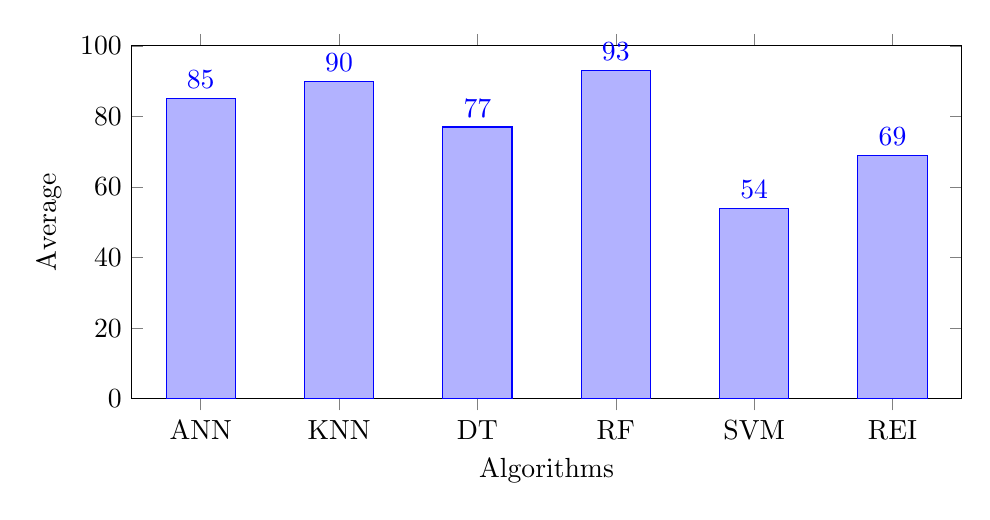
\begin{tikzpicture}
        \begin{axis}[
            ybar,
            symbolic x coords={ANN, KNN, DT, RF, SVM, REI},
            xtick=data,
            nodes near coords,
            ymin=0,
            ymax=100,
            xlabel={Algorithms},
            ylabel={Average},
            bar width=25pt,
            width=1.0\textwidth,
            height=0.5\textwidth
        ]
        \addplot coordinates {(ANN,85) (KNN,90) (DT,77) (RF,93) (SVM,54) (REI,69)};
        \end{axis}
    \end{tikzpicture}
    \caption{Bar graph for average of precision table}
    \label{fig:bar_chart}
\end{figure}

\
\begin{figure}
    \centering
    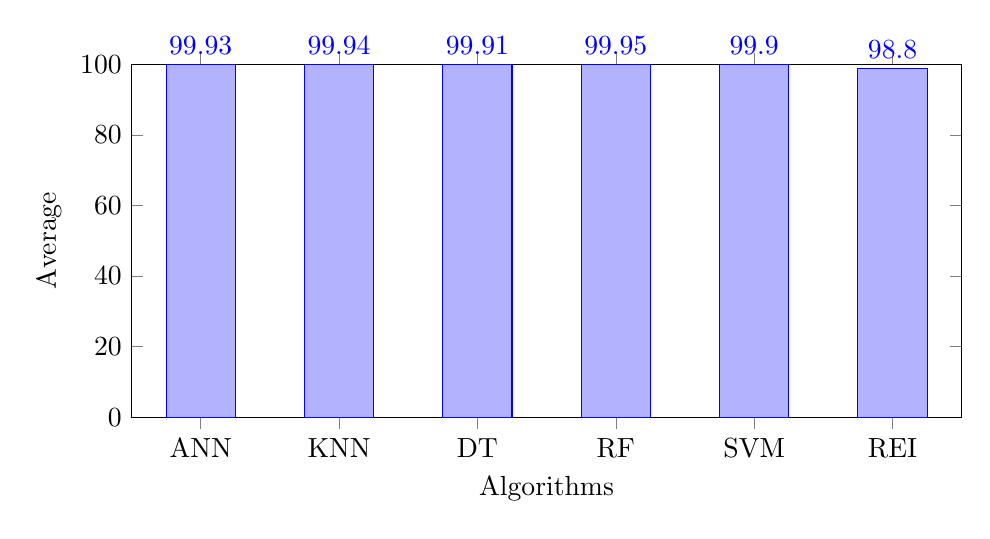
\begin{tikzpicture}
        \begin{axis}[
            ybar,
            symbolic x coords={ANN, KNN, DT, RF, SVM, REI},
            xtick=data,
            nodes near coords,
            ymin=0,
            ymax=100,
            xlabel={Algorithms},
            ylabel={Average},
            bar width=25pt,
            width=1.0\textwidth,
            height=0.5\textwidth
        ]
        \addplot coordinates {(ANN,99.93) (KNN,99.94) (DT,99.91) (RF,99.95) (SVM,99.9) (REI,98.8)};
        \end{axis}
    \end{tikzpicture}
    \caption{Bar graph for average of accuracy table}
    \label{fig:bar_chart}
\end{figure}


\begin{figure}
    \centering
    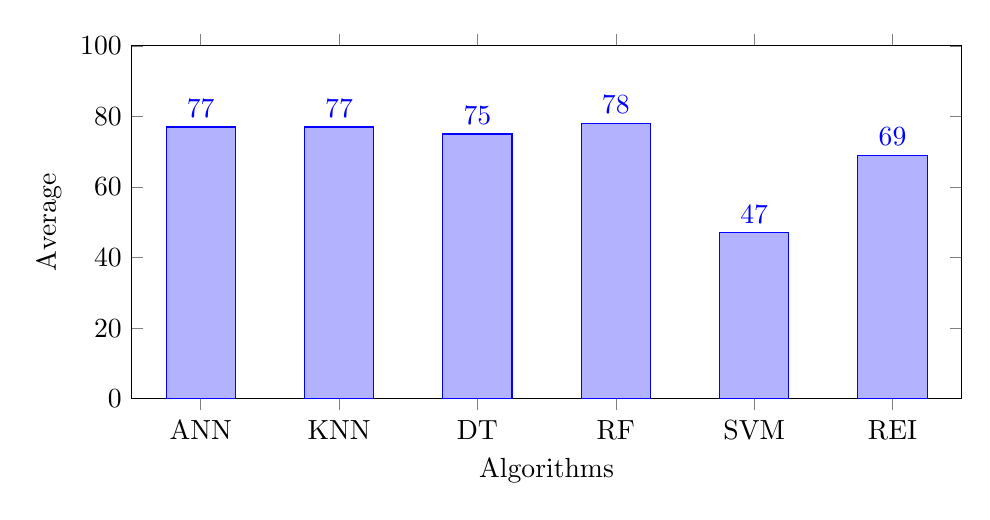
\begin{tikzpicture}
        \begin{axis}[
            ybar,
            symbolic x coords={ANN, KNN, DT, RF, SVM, REI},
            xtick=data,
            nodes near coords,
            ymin=0,
            ymax=100,
            xlabel={Algorithms},
            ylabel={Average},
            bar width=25pt,
            width=1.0\textwidth,
            height=0.5\textwidth
        ]
        \addplot coordinates {(ANN,77) (KNN,77) (DT,75) (RF,78) (SVM,47) (REI,69)};
        \end{axis}
    \end{tikzpicture}
    \caption{Bar graph for average of Recall table}
    \label{fig:bar_chart}
\end{figure}



\begin{figure}
    \centering
    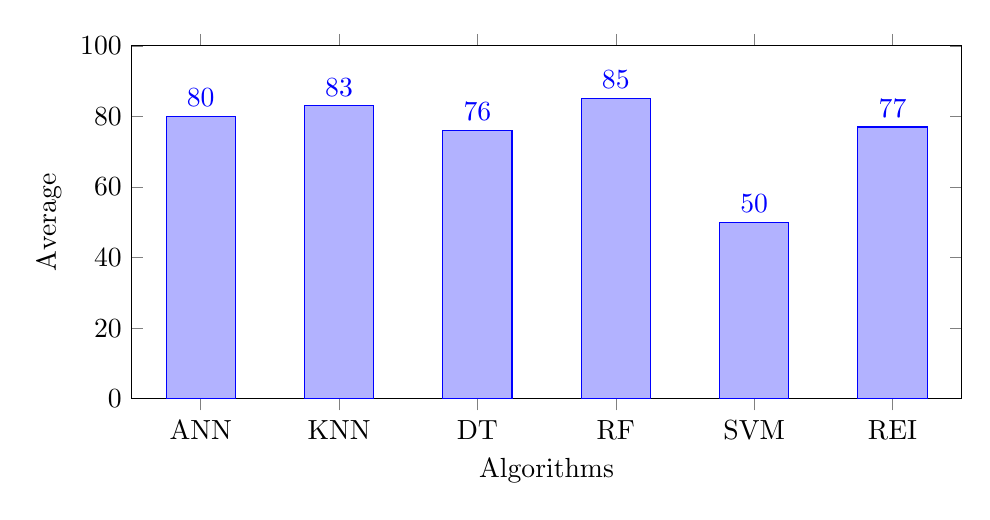
\begin{tikzpicture}
        \begin{axis}[
            ybar,
            symbolic x coords={ANN, KNN, DT, RF, SVM, REI},
            xtick=data,
            nodes near coords,
            ymin=0,
            ymax=100,
            xlabel={Algorithms},
            ylabel={Average},
            bar width=25pt,
            width=1.0\textwidth,
            height=0.5\textwidth
        ]
        \addplot coordinates {(ANN,80) (KNN,83) (DT,76) (RF,85) (SVM,50) (REI,77)};
        \end{axis}
    \end{tikzpicture}
    \caption{Bar graph for average of F1-Score table}
    \label{fig:bar_chart}
\end{figure}




% Conclusion and Future Work
\chapter{Conclusion}
% Include your Conclusion and Future Work content here.


This report comprehensively evaluates six prominent machine learning algorithms—Support Vector Machines (SVM), K-Nearest Neighbors (KNN), Random Forests (RF), Decision Trees (DT), Artificial Neural Networks (ANN), and Reinforcement Learning (RL)—in the context of analyzing financial data. Each algorithm was implemented, and its performance was assessed through precision, accuracy, recall, and F1-score metrics.
\\ \\
Decision Trees and Random Forests offer intuitive and interpretable models but face challenges with overfitting and computational complexity as the number of class labels increases. SVMs and KNNs provide robust classification capabilities, though KNNs can become computationally intensive with large datasets. ANNs excel in capturing complex patterns and non-linear relationships but require significant computational resources and extensive data preprocessing. RL, while not directly comparable through traditional classification metrics, offers a unique approach for sequential decision-making problems by optimizing cumulative rewards through interaction with the environment.
\\ \\
By systematically comparing these algorithms, we identify their strengths and limitations in financial data analysis. Decision Trees and Random Forests are suitable for scenarios requiring interpretability and handling smaller datasets. SVMs and ANNs are ideal for high-dimensional and complex pattern recognition tasks, while KNNs offer simplicity but with increased computational costs for larger datasets. RL stands out for applications involving dynamic and sequential decision-making processes.
\\ \\
Ultimately, the choice of algorithm depends on the specific requirements and constraints of the financial analysis task at hand. This evaluation provides a foundation for selecting the most appropriate machine learning technique, enabling businesses to leverage data-driven insights for strategic decision-making and performance optimization.




\addcon


\end{document}